\documentclass{article}

\usepackage[T1]{fontenc} 
\usepackage[ngerman]{babel}
\usepackage{graphicx}
\bibliography{literatur}
\usepackage{listings}
\usepackage{hyperref}
\usepackage{float}
\usepackage{xcolor}
\definecolor{codegreen}{rgb}{0,0.6,0}
\definecolor{codegray}{rgb}{0.5,0.5,0.5}
\definecolor{codeorange}{rgb}{1,0.49,0}
\definecolor{backcolour}{rgb}{0.95,0.95,0.96}

\lstdefinestyle{mystyle}{
	backgroundcolor=\color{backcolour},   
	commentstyle=\color{codegray},
	keywordstyle=\color{codeorange},
	numberstyle=\tiny\color{codegray},
	stringstyle=\color{codegreen},
	basicstyle=\ttfamily\footnotesize,
	breakatwhitespace=false,         
	breaklines=true,                 
	captionpos=b,                    
	keepspaces=true,                 
	numbers=left,                    
	numbersep=5pt,                  
	showspaces=false,                
	showstringspaces=false,
	showtabs=false,                  
	tabsize=2,
	xleftmargin=10pt,
}

\lstset{style=mystyle}

\begin{document}

\newpage

\section{Implementierung mit Streamlit}

Eine weitere Implementierung des Haar Cascade Klassifizierers wurde 
mit dem Dashboard Framework \textbf{Streamlit} als \textbf{Web-Anwendung} umgesetzt. Das Dashboard enthält
zum einen einen Bereich mit unterschiedlichen Parametern für den 
Haar Cascade Klassifizierer, und zum anderen einen Bereich, in dem 
verschieden Bild-Quellen ausgewählt werden können. Dazu gehört
neben eigenen oder vorinstallierten Bildern auch die Möglichkeit, ein Video
oder das eigene Webcam-Bild zu verwenden.

\begin{figure}[h]
	\begin{center}
 	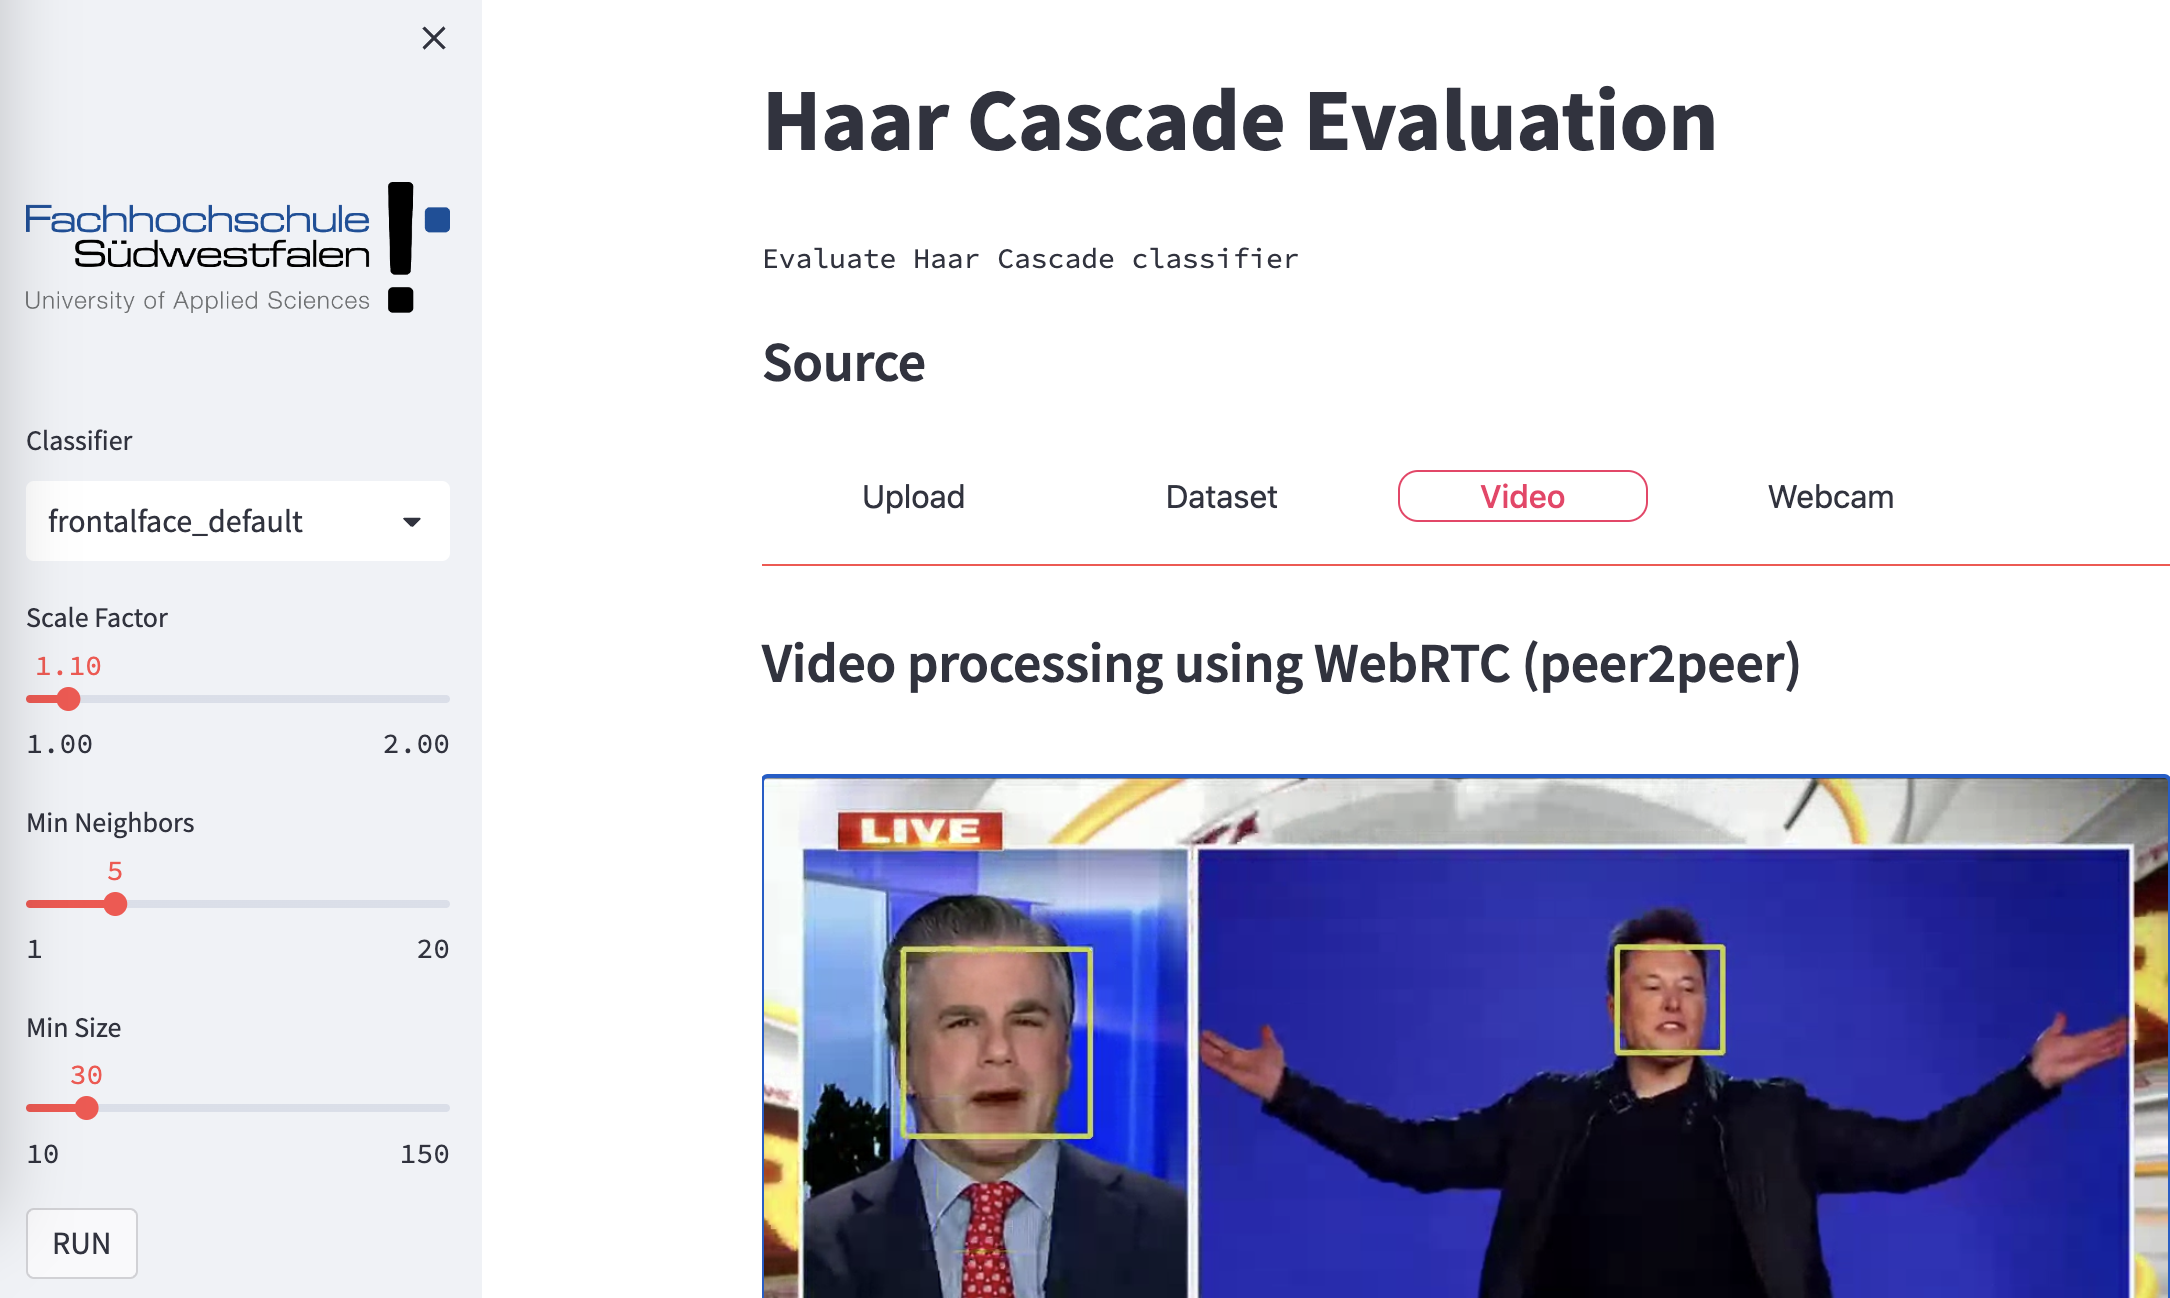
\includegraphics[scale=0.3]{../images/streamlit/video_example.png}
 	\caption{Streamlit Dashboard mit Haar Cascade Klassifizierer}
	\end{center}
\end{figure}

Das Dashboard kann auch als \href{https://jk-fhswf-pki-a22-app-app-codcuk.streamlit.app/}{Demo-Anwendung}
auf der Streamlit-Cloud ausprobiert werden. 

\subsection{Eingabequellen}
Die Anwendung unterstützt diese bereits angesprochenen Eingabemöglichkeiten:

\begin{description}
	\item[Upload]\hfill \\
	Hier kann ein einzelnes Bild hochgeladen und verwendet werden
	\item[Dataset]\hfill \\
	Unter diesem Punkt können mehrere vorkonfigurierte Bilder auf einmal verwendet werden
	\item[Video]\hfill \\
	Bei dieser Option wird ein vorkonfiguriertes Video abgespielt, auf dem der ausgewählte 
	Klassifizierer angewandt wird
	\item[Webcam]\hfill \\
	Hier besteht die Möglichkeit, den Klassifizierer auf die eigene Webcam-Bilder anzuwenden
\end{description}

\subsection{Optionen}
Die verwendeten Optionen zur Konfiguration des Haar Cascade Klassifizierers \textbf{Scale Factor},
\textbf{Min Neighbors} und \textbf{Min Size} wurden bereits in den vorherigen Abschnitten im Rahmen der
Tkinter Anwendung beschrieben. 

\subsection{Code}
Der Programmcode für die Implementierung des Streamlit-Dashboards ist auf die folgenden Quelldateien verteilt:

\begin{lstlisting}[language=Python]
# Hauptanwendung und Einstiegspunkt
app.py
# Funktion zur Ausfuehrung des eigentlichen Klassifizierers
pki_a22_app/haarcascades/haarcascades.py
# Interface fuer die unterschiedlichen Eingabequellen
pki_a22_app/dashboard/sources.py
# Eingabequelle mit einem einzelnen hochladbarem Bild
pki_a22_app/dashboard/source_upload.py
# Eingabequelle mit Auswahl eines Datensatzes mit mehreren Bildern
pki_a22_app/dashboard/source_dataset.py
# Eingabequelle zum Abspielen eines voreingestellten Videos
pki_a22_app/dashboard/source_video.py
# Eingabequelle bei der die eigene Webcam verwendet wird
pki_a22_app/dashboard/source_webcam.py
# Utility Modul, das vor allem Funktionen fuer Datei-Operationen enthaelt
pki_a22_app/utils/file_loader.py
\end{lstlisting}

\section{Organisation}

Besonders zu Beginn war es sehr hilfreich, eine Kollaborations-Plattform 
für das Projekt einzurichten, über die die unterschiedlichsten Informationen
organisatorischer Natur ausgetauscht werden konnten. 
Wir haben uns für den Einsatz eines Miro-Boardes entschieden. das wir 
unter anderem nutzten für:

\begin{itemize}
\item Terminfindung
\item Pinnwand
\item Brainstorming
\item Zeitplanung
\item Wireframes
\end{itemize}

\begin{figure}[ht]
	\begin{center}
 	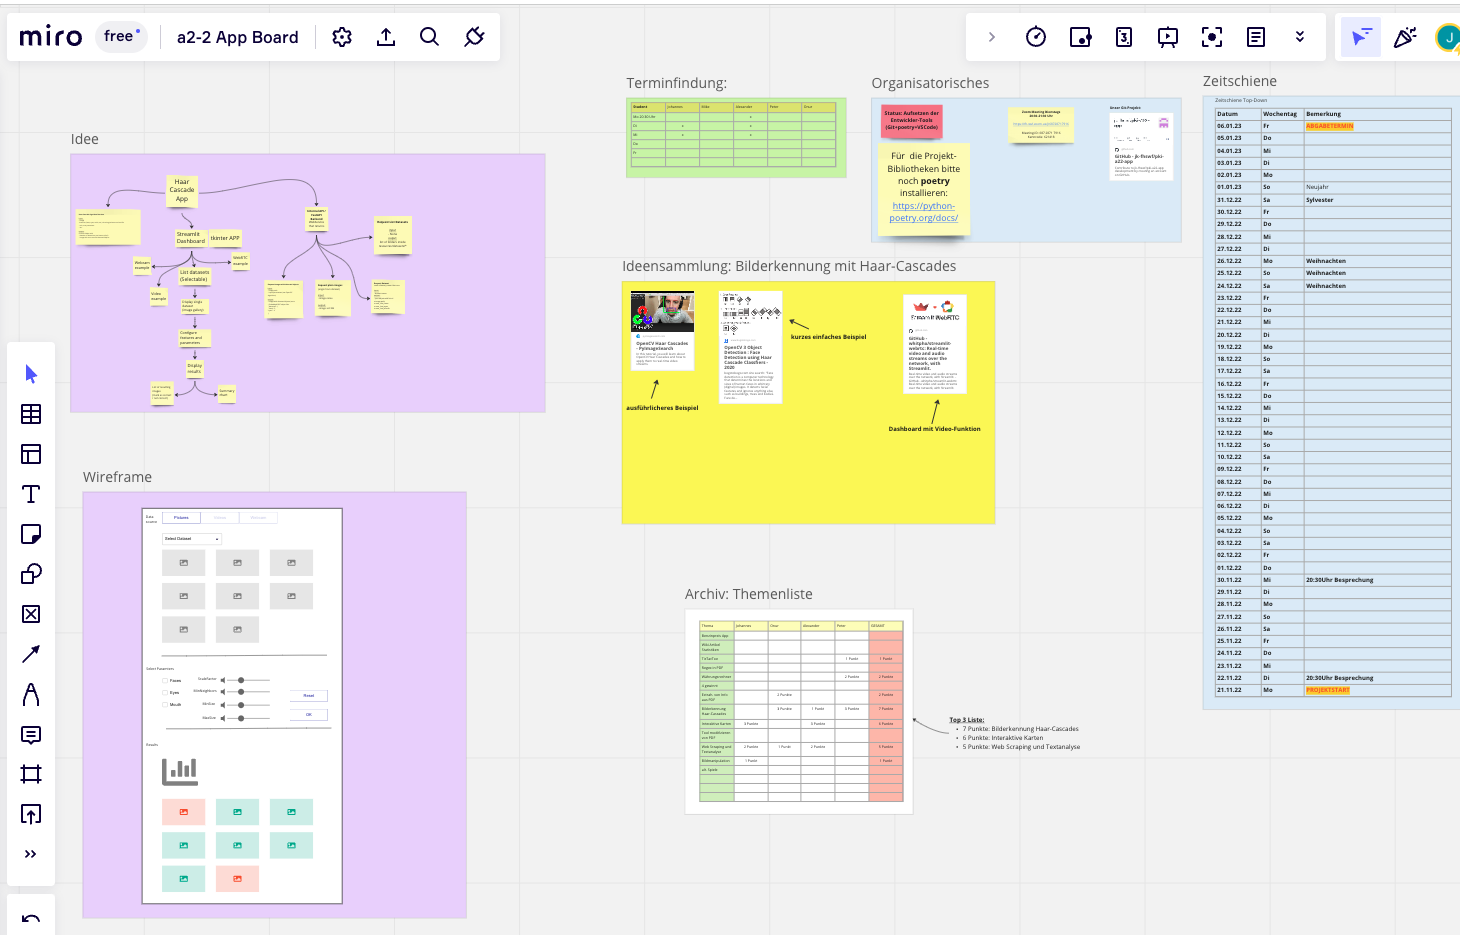
\includegraphics[scale=0.25]{../images/miro_board.png}
 	\caption{Miro-Board für organisatorische Aufgaben}
	\end{center}
\end{figure}

\section{Continuos Integration}

Um gemeinsam am Programmcode arbeiten zu können, haben wir uns ein Git-basiertes 
Codeverwaltungs-Tool entschieden. Hierfür haben wir auf GitHub ein eigenes
\href{https://github.com/jk-fhswf/pki-a22-app}{Git-Repository} eingerichtet.


\begin{figure}[H]
	\begin{center}
 	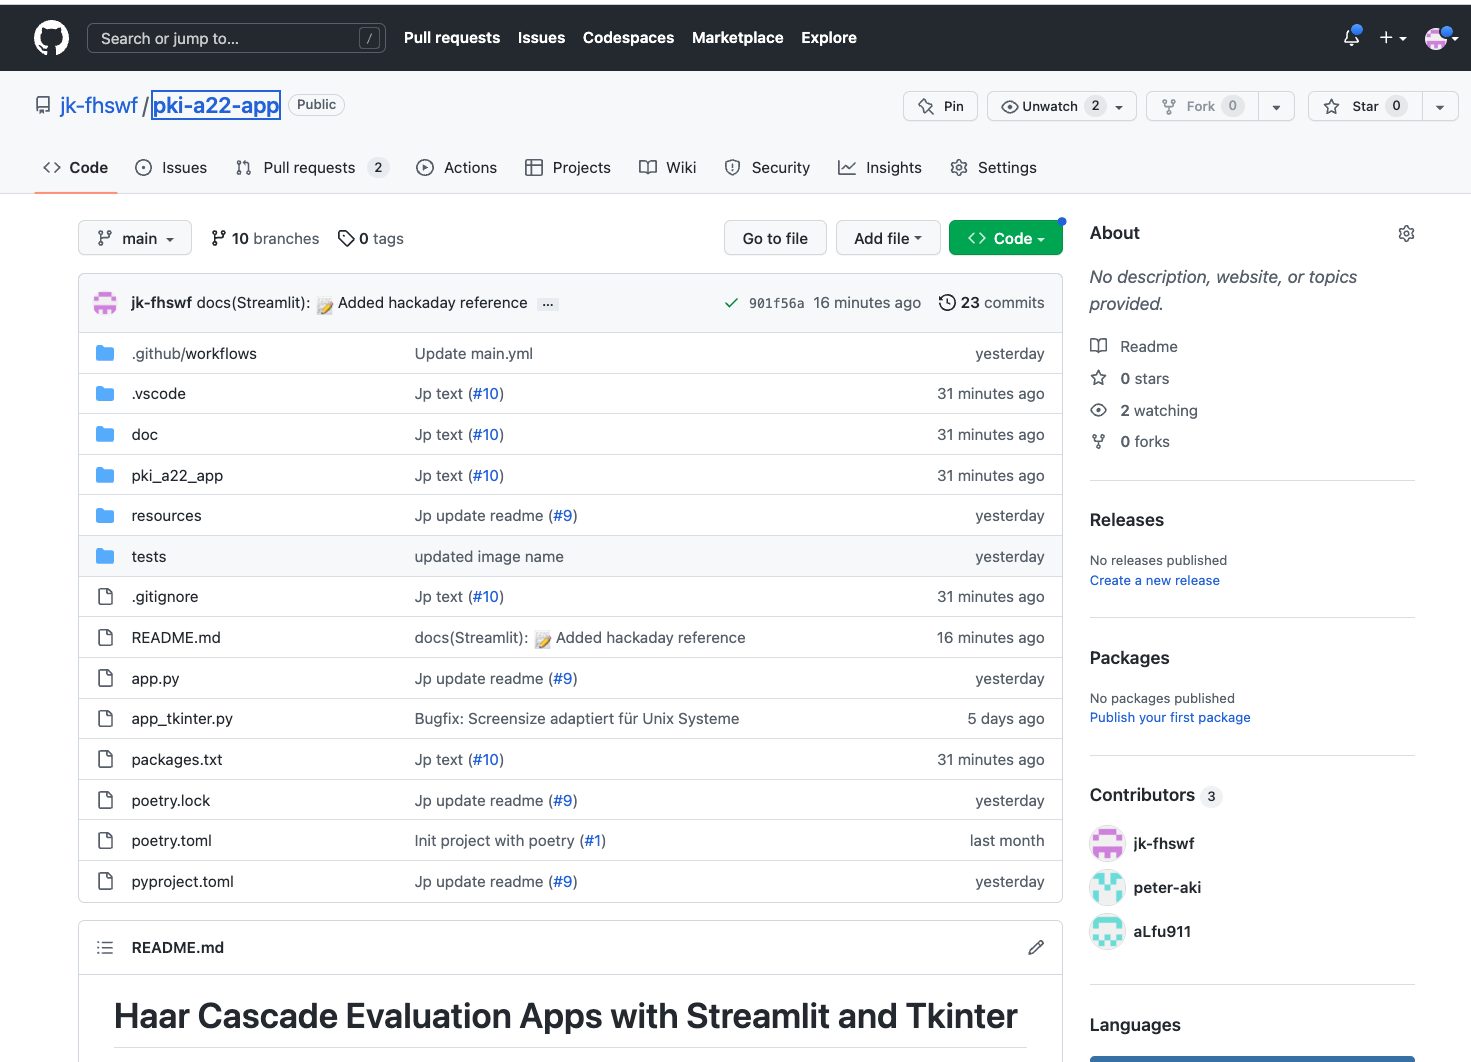
\includegraphics[scale=0.25]{../images/ci_git.png}
 	\caption{Git-Repository auf GitHub}
	\end{center}
\end{figure}

Zur Qualitätssicherung haben wir uns dafür entschieden, für den main-Branch
Pull-Requests zu verwenden und die Erfolgreiche Ausführung eines GitHub-Actions-
Workflows für Unit-Tests vorauszusetzen.

\begin{figure}[H]
	\begin{center}
 	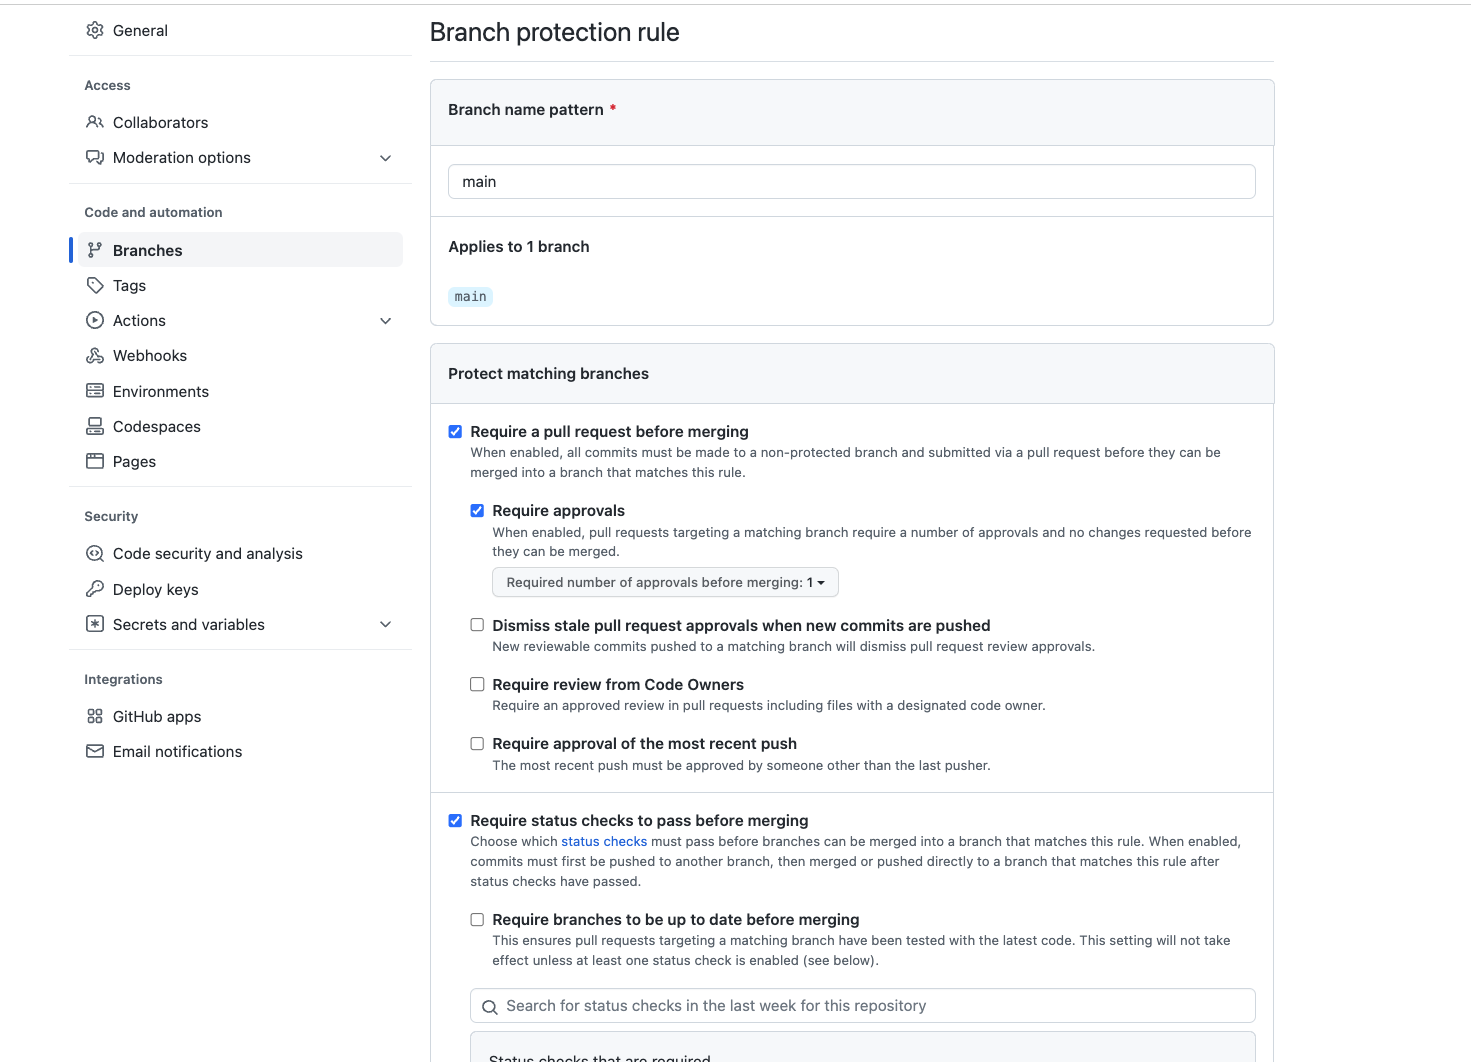
\includegraphics[scale=0.25]{../images/ci_protection.png}
 	\caption{Konfiguration von QA-Optionen}
	\end{center}
\end{figure}


\begin{figure}[H]
	\begin{center}
 	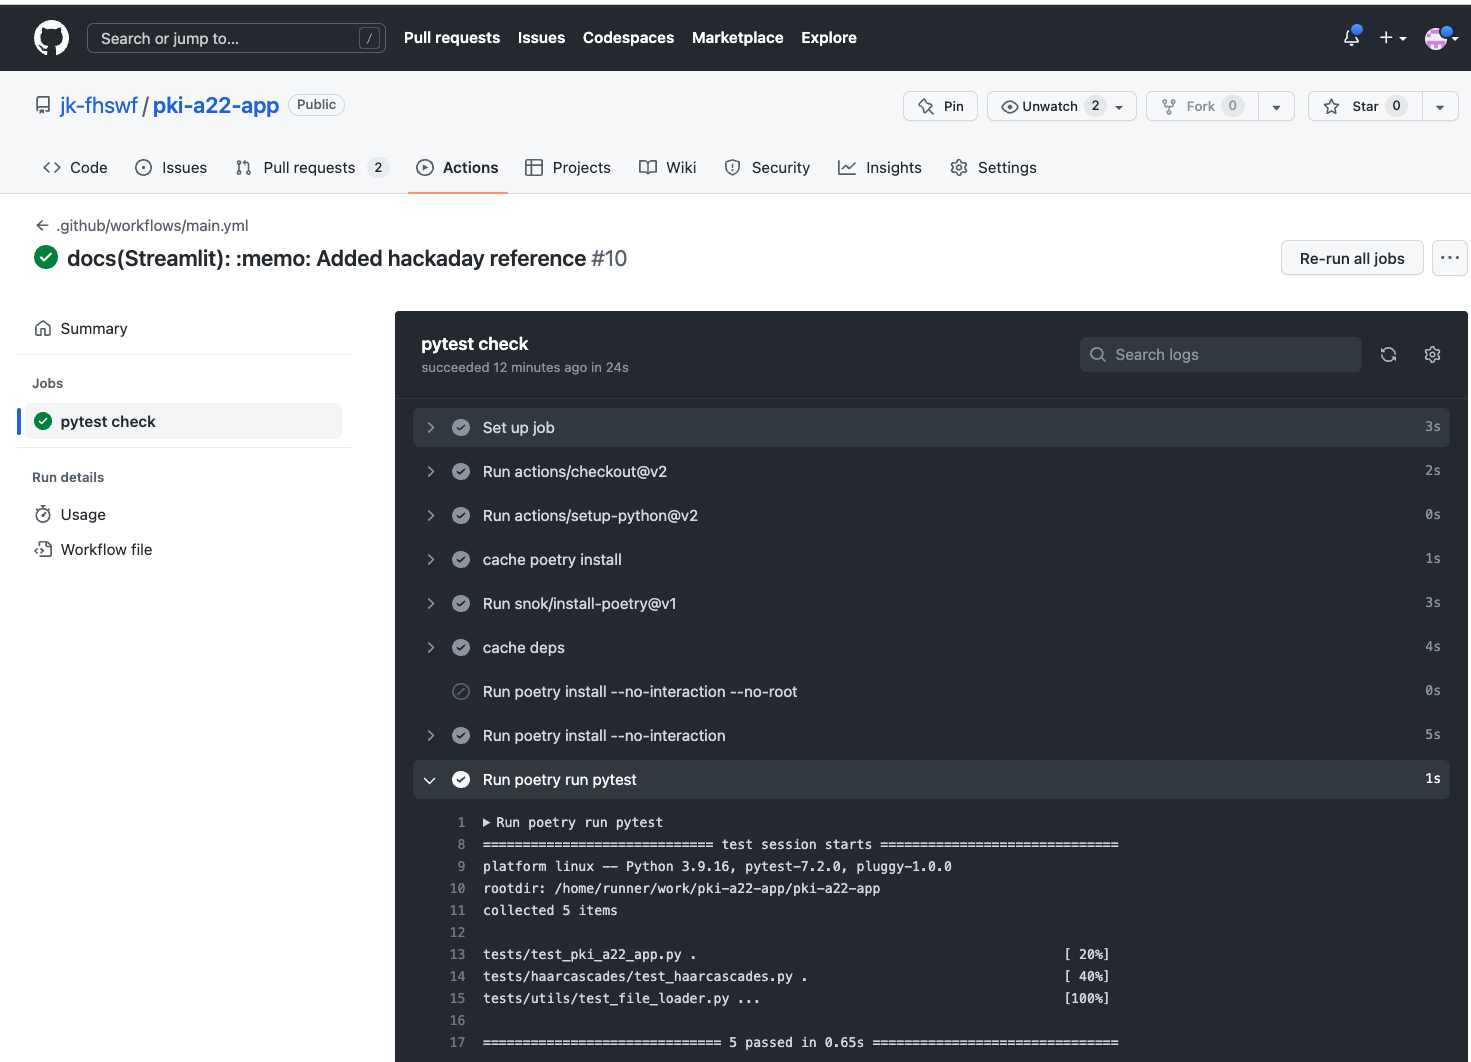
\includegraphics[scale=0.25]{../images/ci_actions.png}
 	\caption{Beispiel Ausführung von Tests mit pytest}
	\end{center}
\end{figure}

\section{Anhang Streamlit Code}


\lstinputlisting[caption=app.py, language=Python]{../../app.py}
\lstinputlisting[caption=haarcascades/haarcascades.py, language=Python]{../../pki_a22_app/haarcascades/haarcascades.py}
\newpage
\begin{figure}
	\centering
	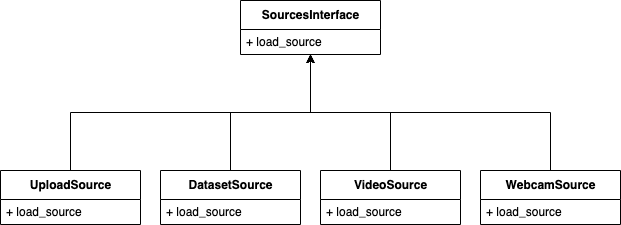
\includegraphics[scale=0.5]{input_sources.png}
	\caption{UML Diagramm für unterschiedliche Source-Typen}
\end{figure}
\lstinputlisting[caption=dashboard/sources.py, language=Python]{../../pki_a22_app/dashboard/sources.py}
\lstinputlisting[caption=dashboard/source upload.py, language=Python]{../../pki_a22_app/dashboard/source_upload.py}
\lstinputlisting[caption=dashboard/source dataset.py, language=Python]{../../pki_a22_app/dashboard/source_dataset.py}
\lstinputlisting[caption=dashboard/source video.py, language=Python]{../../pki_a22_app/dashboard/source_video.py}
\lstinputlisting[caption=dashboard/source webcam.py, language=Python]{../../pki_a22_app/dashboard/source_webcam.py}
\lstinputlisting[caption=utils/file loader.py, language=Python]{../../pki_a22_app/utils/file_loader.py}


\end{document}

 